\chapter{Methodology}
\label{ch:3}
This chapter describes the method the thesis set out to evaluate, D-MTHD, and the change of setting
that turned out to matter. Figure~\ref{fig:schematic} shows the distinction the thesis turns on: in
both settings the same teacher and the same student are used, and only the text on which the student
imitates the teacher differs. Sections~\ref{sec:3.1} to~\ref{sec:3.4} define the committee, the
per-instance weighting, the objective and the specialist teacher exactly as they were audited;
Section~\ref{sec:3.5} defines in-sample and out-of-sample distillation and their controls;
Section~\ref{sec:3.6} states what is measured about the weighting; and Section~\ref{sec:3.7} gives
the training procedure as an algorithm.
\begin{figure}[htbp]
\centering
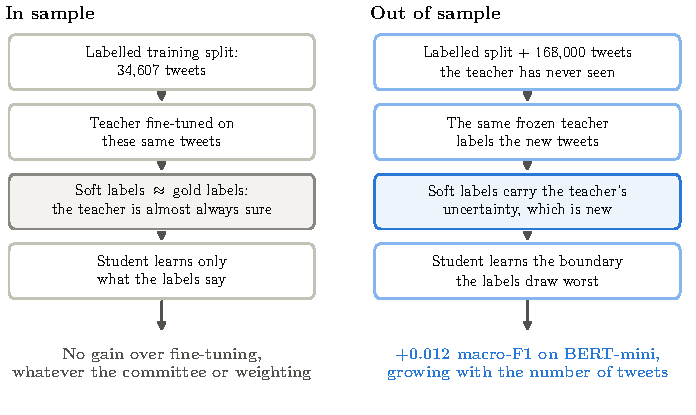
\includegraphics[width=\textwidth]{figures/fig_schematic.pdf}
\caption{In-sample against out-of-sample distillation. The same teacher and student are used in both settings; only the text on which the student imitates the teacher differs. In sample, on the tweets the teacher was fine-tuned on, its soft labels repeat the gold labels; out of sample, on tweets it has never seen, they carry its uncertainty.}
\label{fig:schematic}
\end{figure}
\section{Notation and Committee}
\label{sec:3.1}
Let $x_i$ be a text with majority label $y_i \in \{1,\dots,C\}$. A committee of $K$ teachers
produces logits $z_k(x_i) \in \mathbb{R}^C$ and masked-mean-pooled last-layer states $h_k(x_i) \in
\mathbb{R}^{d_k}$; the student produces $z_s(x_i)$ and $h_s(x_i) \in \mathbb{R}^{d_s}$, plus an
auxiliary irony head $z_s^{\text{irony}}(x_i) \in \mathbb{R}^2$. $W_k \in \mathbb{R}^{d_k \times
d_s}$ is a learned projection from the student width to teacher $k$'s width; $T$ is the distillation
temperature and $\tau$ the weight temperature.

Teachers are \emph{task-adapted}: each is initialised from a specialist checkpoint and fine-tuned on
the target training split, so that every committee member shares the task's label space. Without
this step a sarcasm model's logits are not comparable with an abuse model's and cannot enter a KL
term. The homogeneous committee $\mathcal{K}_{\text{homo}}$ is BERT-large \cite{devlin2019bert},
HateBERT \cite{caselli2021hatebert} and a Twitter irony RoBERTa \cite{barbieri2020tweeteval,
liu2019roberta}: a general encoder, a specialist in abuse that says what it means, and a specialist
in saying one thing and meaning another. The heterogeneous committee adds DeBERTa-v3-base
\cite{he2023debertav3}. The third committee adds the implicit specialist of Section~\ref{sec:3.4}.
Teachers are frozen after adaptation and their outputs cached once on every split the student will
train on; the student never sees a teacher at run time.
\section{Per-Instance Reliability}
\label{sec:3.2}
For each training instance the committee is weighted by how reliable each teacher is on it:

\begin{equation}
\ell_k(i) = \mathrm{CE}\big(\mathrm{softmax}(z_k(x_i)),\, y_i\big), \qquad
w_k(i) = \frac{\exp(-\ell_k(i)/\tau)}{\sum_{j} \exp(-\ell_j(i)/\tau)} .
\end{equation}

$w_k(i)$ is the posterior probability that teacher $k$ is the right expert for $x_i$ under a uniform
prior and a likelihood $p(y_i \mid k, x_i)^{1/\tau}$: at $\tau = 1$ it is Bayesian model averaging
over the committee on that instance; $\tau \to \infty$ recovers uniform averaging and $\tau \to 0$
hard selection of the single best teacher. Per-batch weighting, as in earlier work, replaces
$\ell_k(i)$ by its batch mean. Because the teachers are frozen and cached, $w_k(i)$ is a fixed
function of the data: it varies across instances and never across epochs or seeds, so ``dynamic''
means instance-adaptive and nothing else.
\section{Objective}
\label{sec:3.3}
\begin{equation}
\bar p(i) = \sum_k w_k(i)\, \mathrm{softmax}\!\big(z_k(x_i)/T\big), \qquad
\mathcal{L}_{\mathrm{KL}}(i) = T^2\, \mathrm{KL}\!\big(\bar p(i)\,\|\,\mathrm{softmax}(z_s(x_i)/T)\big),
\end{equation}

\begin{equation}
\mathcal{L}_{\mathrm{hid}}(i) = \sum_k w_k(i)\, \big\| W_k h_s(x_i) - h_k(x_i) \big\|_2^2, \qquad
\mathcal{L}_{\mathrm{irony}}(i) = T^2\, \mathrm{KL}\!\big(\mathrm{softmax}(z_{\text{irony}}(x_i)/T)\,\|\,\mathrm{softmax}(z_s^{\text{irony}}(x_i)/T)\big),
\end{equation}

\begin{equation}
\mathcal{L} = \frac{1}{B}\sum_i \Big[\alpha\, \mathcal{L}_{\mathrm{KL}}(i) + \beta\, m_i\, \mathrm{CE}(z_s(x_i), y_i)
 + \gamma\, \mathcal{L}_{\mathrm{hid}}(i) + \delta\, \mathcal{L}_{\mathrm{irony}}(i)\Big],
\end{equation}

with $\alpha = \beta = 0.4$, $\gamma = 0.2$, $\delta = 0.3$, $T = 4$ and $\tau = 1$ unless stated,
and $m_i \in \{0, 1\}$ a label mask that is 1 on labelled rows and 0 on the unlabelled rows of
Section~\ref{sec:3.5}. The irony teacher cannot join the committee, because its label space is irony
against non-irony, so its softened output is distilled into a second head on the student's pooled
state; the head is discarded at inference and exists to shape the shared representation. Uniform
multi-teacher distillation sets $w_k(i) = 1/K$; single-teacher distillation uses BERT-large alone;
fine-tune-only sets $\alpha = \gamma = \delta = 0$. Training: 6 epochs, AdamW
\cite{loshchilov2019decoupled} at $3 \times 10^{-5}$ ($10^{-3}$ for the BiLSTM), 10 per cent warm-up
and linear decay, batch 32, gradient clipping at 1.0, mixed precision on GPU, best validation
macro-F1 epoch kept, early stopping with patience 2, implemented in PyTorch and Transformers
\cite{paszke2019pytorch, wolf2020transformers}.
\section{The Implicit Specialist and Its Controls}
\label{sec:3.4}
No public checkpoint and neither established corpus holds knowledge of abuse by implication, so a
committee assembled from them cannot route to it. We therefore train the fourth member: HateBERT
fine-tuned on the implicit benchmark of Section~\ref{sec:4.2}, then task-adapted onto the tweet
corpus like every other teacher, its classification head re-initialised for the six-class label
space. It forms its own committee, $\mathcal{K}_{\text{spec}} = \mathcal{K}_{\text{homo}} \cup
\{\text{specialist}\}$, so that its effect is a three-seed comparison of two full committees rather
than a single ablation. Two controls accompany it, fixed before it was trained. The first distils
from the specialist alone, asking whether the committee contributes anything the specialist does
not. The second fine-tunes the same student on the implicit corpus and then on the tweet task with
no teacher, asking whether the knowledge, if any arrives, came from distillation or from the data.
\section{In Sample and Out of Sample}
\label{sec:3.5}
Every objective above is evaluated in two settings that differ only in where the teacher's function
is sampled. \emph{In sample}, the student is trained on the labelled split $\mathcal{D}$, the
teachers' outputs are cached on $\mathcal{D}$, and $\mathcal{D}$ is the split the teachers were
fine-tuned on. \emph{Out of sample}, an unlabelled transfer set $\mathcal{U}$ of texts outside every
teacher's training split is appended to $\mathcal{D}$; on $x_u \in \mathcal{U}$ the label mask $m_u
= 0$ removes the hard-label term, and the student trains from $\alpha\, \mathcal{L}_{\mathrm{KL}}(u)
+ \gamma\, \mathcal{L}_{\mathrm{hid}}(u) + \delta\, \mathcal{L}_{\mathrm{irony}}(u)$ alone. Nothing
else changes: the same objective, teachers, student, epochs and learning rate. The construction of
$\mathcal{U}$ is in Section~\ref{sec:4.4}; it is shuffled once with a fixed seed so that its
prefixes are nested subsets, which is what lets Section~\ref{sec:5.8} vary its size with everything
else fixed.

Two controls separate what the soft labels carry from what more text and more updates carry. The
\emph{hard-label} control replaces $\bar p(u)$ by the committee's $\arg\max$ and trains the transfer
rows with cross-entropy alone. The \emph{matched-steps} controls fine-tune the student with no
teacher for as many updates as a transfer arm takes (13 epochs for the 42,013-row set, 35 for the
168,000-row set), early stopping off and the best validation epoch kept, so that optimisation length
is held equal rather than argued away.

Out of sample, the reliability of Section~\ref{sec:3.2} has no label to be scored against, so we
also test a reliability the teachers cannot have memorised. Let $\mathcal{V}$ be the validation
split, $c_k(v) \in \{0, 1\}$ whether teacher $k$ is correct on $v \in \mathcal{V}$, and $N_k(x)$ the
$m$ validation texts nearest $x$ by cosine similarity in teacher $k$'s own pooled space. Then

\begin{equation}
r_k(x) = \frac{1 + \sum_{v \in N_k(x)} c_k(v)}{m + 2}, \qquad
w_k(x) = \frac{r_k(x)^{1/\tau}}{\sum_j r_j(x)^{1/\tau}},
\end{equation}

with $m = 20$ and $\tau = 1$: the weight is proportional to the teacher's local out-of-sample
accuracy, defined on labelled and unlabelled rows alike. It is a control, not a proposal:
Section~\ref{sec:5.4} sets its ceiling before any student trains on it.
\section{What Is Measured About the Weighting}
\label{sec:3.6}
A committee of specialists is only a committee if the weights go somewhere. For each teacher we
report the \emph{routing contrast}: its mean weight on instances of the class that holds indirect
abuse minus its mean weight on the classes that name their target, with a percentile bootstrap
interval over 2,000 resamples, measured in the committee the students actually trained with. With
tens of thousands of training instances almost any contrast excludes zero, so its size is read
against the uniform weight $1/K$. And because the weights are a fixed function of the data, the
sweep over $\tau$ reaches 0.05, where they are as sharp as the reliability signal allows.

\section{Training Procedure}
\label{sec:3.7}
Algorithm~\ref{alg:training} gives the procedure shared by every run. In-sample runs use an empty
transfer set; fine-tune-only runs skip the teachers and train on the labelled split with cross-entropy
alone.

\begin{algorithm}[htbp]
\caption{Distillation in and out of sample.}
\label{alg:training}
\begin{algorithmic}[1]
\Require labelled split $\mathcal{D}$; unlabelled transfer set $\mathcal{U}$, empty in sample; teacher
  checkpoints $M_1, \dots, M_K$; irony teacher $M_{\mathrm{irony}}$; pre-trained student $S$
\For{$k = 1, \dots, K$}
  \State fine-tune $M_k$ on $\mathcal{D}$, keep its best validation epoch, and freeze it \Comment{task adaptation}
\EndFor
\For{each text $x \in \mathcal{D} \cup \mathcal{U}$}
  \State cache $z_k(x)$ and $h_k(x)$ for every teacher $k$, and $z_{\mathrm{irony}}(x)$
\EndFor
\State set the label mask $m_x = 1$ for $x \in \mathcal{D}$ and $m_x = 0$ for $x \in \mathcal{U}$
\For{epoch $= 1, \dots, E$}
  \For{each minibatch $B$ drawn from $\mathcal{D} \cup \mathcal{U}$}
    \State compute $z_s(x)$, $h_s(x)$ and $z^{\mathrm{irony}}_s(x)$ for $x \in B$
    \State compute the weights $w_k(x)$ of Section~\ref{sec:3.2}, or of Section~\ref{sec:3.5} out of sample
    \State compute the loss of Section~\ref{sec:3.3} with the mask $m_x$ and update $S$ and $W_1, \dots, W_K$
  \EndFor
  \State evaluate macro-F1 on the validation split and keep the best epoch
\EndFor
\State \Return $S$, discarding the projections $W_k$ and the irony head
\end{algorithmic}
\end{algorithm}
